\noindent \textred{4.} Finding the median of an unordered array in O(n) (Part I). Let’s consider the algorithm \ref{alg:findMedian},

\begin{algorithm}
\caption{\textbf{FindMedian}$(L)$} \label{alg:findMedian}
\begin{algorithmic}
\Require $L$ as input list containing $n$ real numbers
\Ensure The median of $L$ as $m$
\If{$n < 10$}
    \State Sort $L$ and return the median $m$
\EndIf
\State Divide $L$ into $\frac{n}{5}$ lists of size 5 each
\State Sort each list, let $i^{th}$ list be $a_i \leq a_i' \leq b_i \leq c_i \leq c_i', i = 1, 2, \dots, \frac{n}{5}$
\State Recursively find median of $b_1, b_2, \dots, b_\frac{n}{5}$, call it $b*$
\State Reorder indices so that $b_1, b_2, \dots, b_\frac{n}{10} \leq b* < b_{\frac{n}{10} + 1}, \dots, b_\frac{n}{5}$
\State Define $A$ and $C$ as shown in the figure (both $A$ and $C$ have approximately $\frac{3}{10} n$ elements)
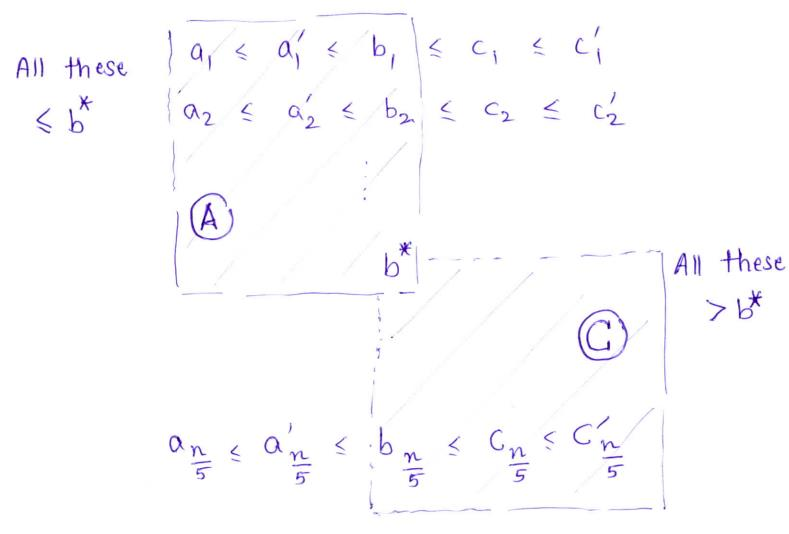
\includegraphics[width=0.6\linewidth]{HWs/HW3/HW03_included.jpg}
\State Drop $A$ and $C$ from the original list $L$, to get a new list $L'$, with $n - \frac{3}{10}n - \frac{3}{10}n = \frac{2}{5}n $ elements
\State Find median of remaining $L'$ recursively and return it as $m$.
\end{algorithmic}
\end{algorithm}

\noindent Note that there could be some corner cases to consider, like $n$ is not a multiple of 5 (can be fixed by padding), or the number of elements in $A$ or $C$ is inaccurate. However, as long as $n$ is large enough, this little inaccuracy will not infect the analysis of complexity. \\
(a) Let $T(n)$ be the running time of Algo.\ref{alg:findMedian}, find the recurrence formula, and then solve it. \\
\textblue{
The Algo.\ref{alg:findMedian} recursively calls itself twice, with input size of $\frac{1}{5} n$ and $\frac{2}{5} n$ respectively. Moreover, it calls a sorting algorithm on $\frac{1}{5} n$ lists, each of size 5, which contributes a time complexity of $\frac{1}{5} n \cdot C \sim O(n)$. The rest part of the Algo.\ref{alg:findMedian} has a constant time complexity. Therefore, the recurrence formula is 
\begin{equation} \label{eq:HW03_04_recursion}
    T(n) \simeq T(\frac{n}{5}) + T(\frac{2 n}{5}) + O(n),
\end{equation}
which we can analyse with recursion tree as in \figref{fig:HW03_04_tree}. We can see that the time complexity of $T(n)$ is almost the same as that of $S(n)$:\\
\begin{equation}
    S(n) = \frac{3}{5} S(n) + O(n),
\end{equation}
except for the total recursion level number on each branch. Moreover, the total recursion level of $T(n)$ must be less than that of $S(n)$ since $\max(\log_{\frac{5}{2}} n, \log_5 n) < \log_{\frac{5}{3}} n$. Thus we have $T(n) = O(S(n))$. 
To solve $S(n)$, we can apply Master's method where $a=1$, $b=\frac{5}{3}$ and $f(n) = n$ which indicates that $S(n) = O(n)$. Or we can simply sum up all the cost of $S(n)$:
\[
\begin{aligned}
    S(n) &\leq \left[ 1 + \frac{3}{5} + (\frac{3}{5})^2 + \cdots + (\frac{3}{5})^{+\infty} \right] \cdot n \\
    &= \frac{1}{1 - \frac{3}{5}} \cdot n = \frac{5}{2} n \implies S(n) = O(n)
\end{aligned}
\]
Combined with $T(n) = O(S(n))$, we conclude that $\underline{T(n) = O(n)}$.
}

\begin{figure}[!ht]
    \centering
    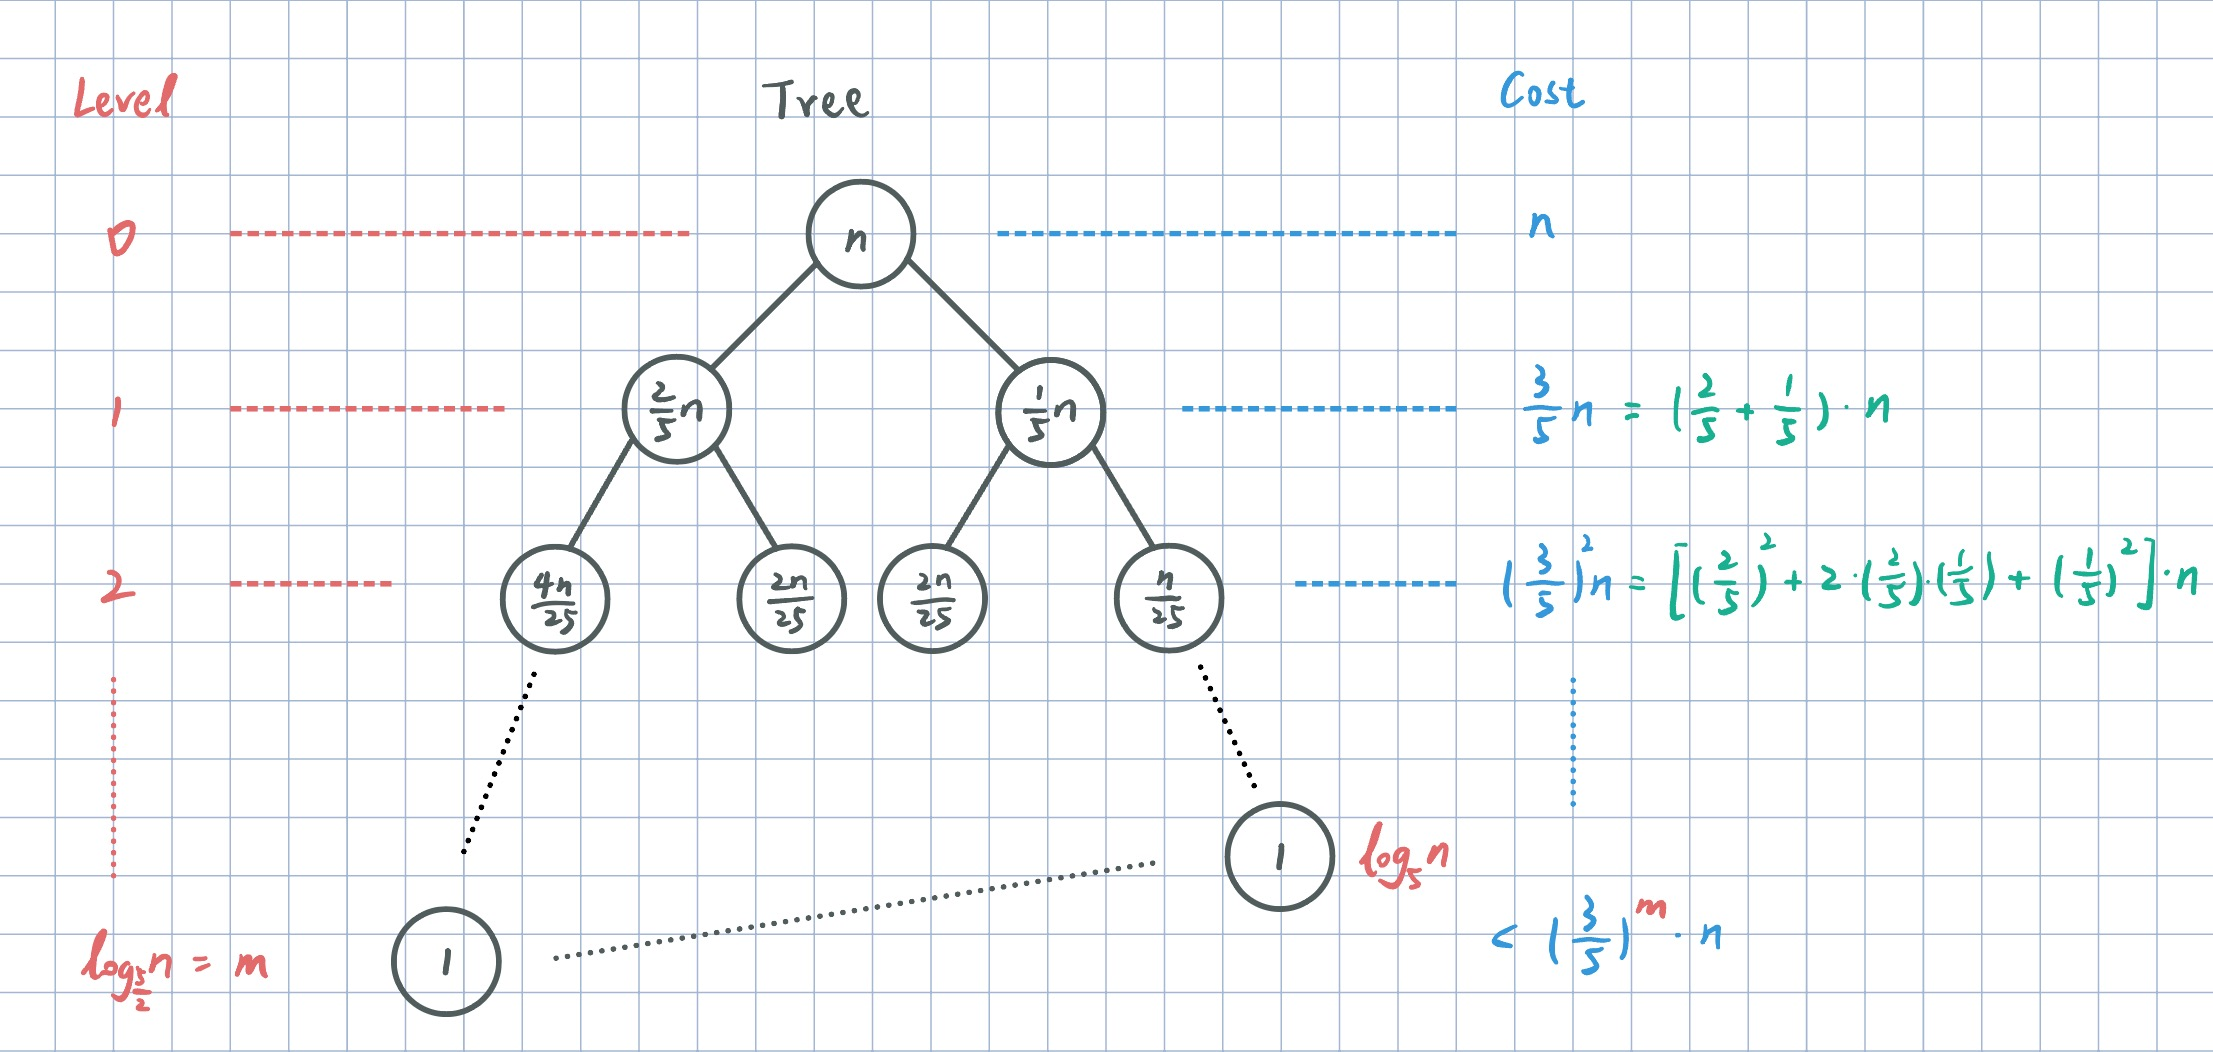
\includegraphics[width=0.9\linewidth]{HWs/HW3/HW03_04_a.jpg}
    \caption{Recursion tree of $T(n)$ in Eq.\eqref{eq:HW03_04_recursion}}
    \label{fig:HW03_04_tree}
\end{figure}

\noindent (b) Is this algorithm correct? If yes, try to prove it; otherwise, find a counter case (like the true median is in $A$ or $C$ and is dropped). \\
\textblue{
\underline{No, it is not correct}. Consider a simple case that the original list $L$ is $[1, 2, 3, \dots, 15]$. According to Algo.\ref{alg:findMedian}, we first divide $L$ into $\frac{15}{5} = 3$ lists, which are $[1, 2, \dots, 5]$, $[6, 7, \dots, 10]$, and $[11, 12 ,\dots, 15]$. Since they are all in sort, we don't need to bother finding the median of $[b_1, b_2, b_3]$ or re-indexing these sub-lists. Next, according to the definition of $A$ and $C$, the true median, 8 , is discard, as shown in \figref{fig:HW03_04_8}.
Therefore, we have described a counter case. %to demonstrated the incorrectness of the algorithm.
\begin{figure}[!h]
    \centering
    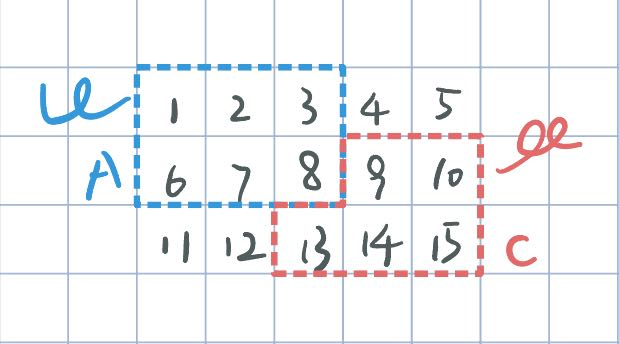
\includegraphics[width=0.3\linewidth]{HWs/HW3/HW03_04.jpg}
    \caption{}
    \label{fig:HW03_04_8}
\end{figure}
}
